\documentclass{beamer}
\usepackage[utf8]{inputenc}
\usepackage{lmodern}
\usepackage[brazil]{babel}
\usepackage{graphicx}
\usepackage{tcolorbox}
\tcbuselibrary{skins}
\usetheme{Madrid}

% -------------------------------------------------
% Identidade Visual - Centro Paula Souza
% -------------------------------------------------
\definecolor{cpsred}{RGB}{153,0,0}      % Vermelho institucional
\definecolor{cpsgray}{RGB}{85,85,85}    % Cinza técnico

\usecolortheme[named=cpsred]{structure}
\setbeamercolor{title}{fg=white,bg=cpsred}
\setbeamercolor{frametitle}{fg=white,bg=cpsred}
\setbeamercolor{structure}{fg=cpsred}
\setbeamercolor{normal text}{fg=black,bg=white}
\setbeamercolor{itemize item}{fg=cpsred}

\usepackage{ragged2e}
\usepackage{hyperref}

\setbeamertemplate{headline}{} 

% -------------------------------------------------
% Rodapé padrão
% -------------------------------------------------
\setbeamertemplate{footline}[frame number]
\addtobeamertemplate{footline}{
  \hfill\usebeamercolor[fg]{frametitle}{\hspace{-1.5cm}\scriptsize Ana Flávia - Geovanna - Miguel - Vinícius - Vitor}\hspace{1cm}
}{}

% -------------------------------------------------
% Informações principais
% -------------------------------------------------
\title[Apresentação do projeto Luna]{\textbf{ Luna }}
\author{Ana Flávia - Geovanna - Miguel - Vinícius - Vitor}
\date{}

% -------------------------------------------------
% Documento
% -------------------------------------------------
\begin{document}

% Capa
\begin{frame}
    \centering
    \centering
    \vspace{1cm}
    {\color{cpsred}\Huge\textbf{Luna}}\\[0.8cm]
    {\Large Ana Flávia - Geovanna - Miguel}\\[0.4cm]
    {\Large Vinícius - Vitor}\\[0.4cm]
    \textcolor{cpsgray}{Centro Paula Souza}\\[0.2cm]
    \textcolor{cpsgray}{FATEC Registro}
\end{frame}

% Sumário
\begin{frame}{Sumário}
\tableofcontents
\end{frame}

% -------------------------------------------------
% SEÇÕES E SLIDES
% -------------------------------------------------

\section{Pitch}
\begin{frame}{Pitch}
\centering
{\Large\textbf{\textcolor{cpsred}{Apresentação do Pitch}}}\\[0.4cm]
\textcolor{cpsgray}{Resumo visual e conceitual do projeto Luna}\\[0.8cm]
\vspace{0.3cm}

\begin{center}
\begin{tcolorbox}[
    enhanced,
    colback=white,
    colframe=cpsred,
    boxrule=1pt,
    arc=6pt,
    width=0.7\linewidth,
    center,
    halign=center,
    valign=center,
    shadow={0mm}{-0.5mm}{0mm}{cpsgray!30},
    top=10pt,
    bottom=10pt
]
\centering
\large
\href{https://www.youtube.com/watch?v=s2I0XjJmF1Y}{PITCH}
\end{tcolorbox}
\end{center}
\vspace{1cm}

\centering
{\small O pitch sintetiza a proposta do \textbf{Luna}, um projeto que utiliza \textbf{Inteligência Artificial Generativa} para auxiliar professores na criação de planos de aula personalizados para crianças com TDAH.}

\end{frame}

% --- Frame introdução

\section{Introdução}
\begin{frame}{Introdução}
    \begin{columns}
        \begin{column}{0.6\textwidth}
    \justifying
    \begin{itemize}
        \item TDAH impacta aprendizagem e socialização infantil, com desafios contínuos no diagnóstico e adaptação escolar;
        
        \item Luna utiliza IA para ajudar professores a criarem planos de aula personalizados baseado  no hiperfoco de cada aluno;
        
        \item Alunos acompanham suas atividades, enquanto responsáveis e professores monitoram o progresso através de relatórios em formato de gráficos;
    \end{itemize}
\end{column}
        
        \begin{column}{0.35\textwidth}
            \centering
            \fbox{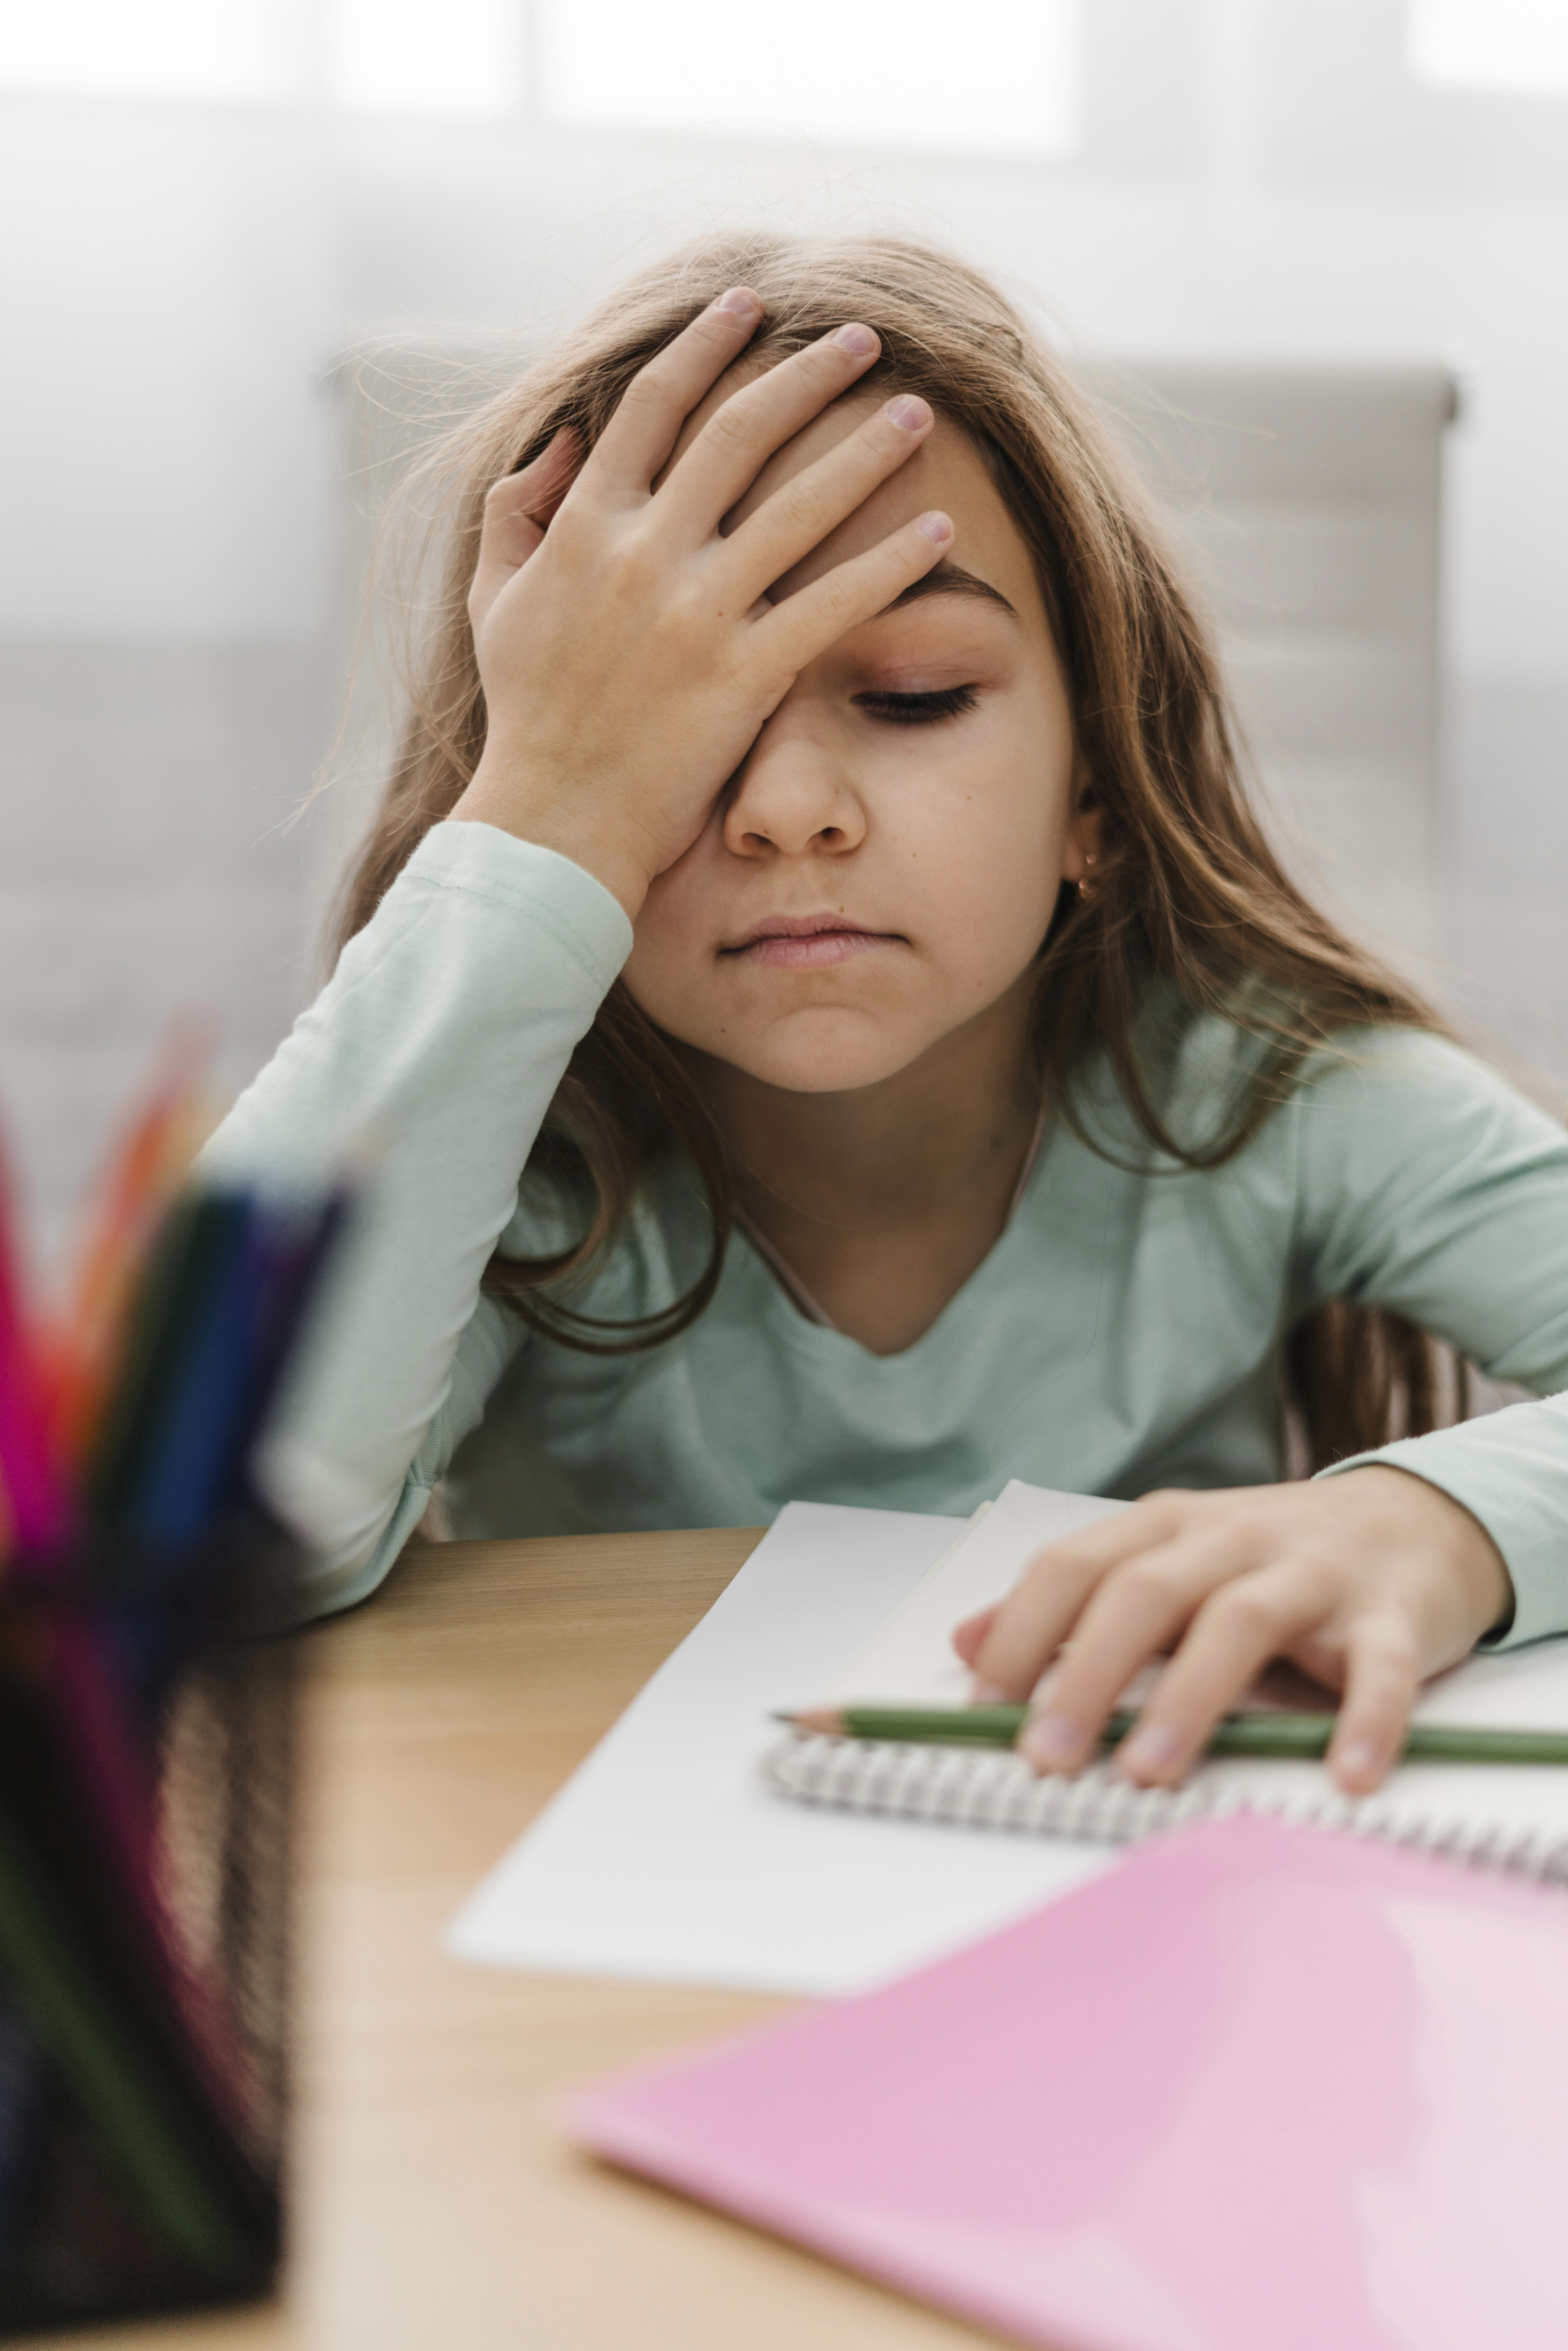
\includegraphics[width=0.9\textwidth]{img1.jpg}}
            \\[0.3cm]
            \tiny\textcolor{cpsgray}{Fonte: Imagem gerada por IA (Freepik), 2025}
        \end{column}
    \end{columns}
\end{frame}

% --- Frame estado da arte

\section{Estado da arte}
\begin{frame}{Estado da arte}
    \begin{columns}
        \begin{column}{0.35\textwidth}
            \centering
            \fbox{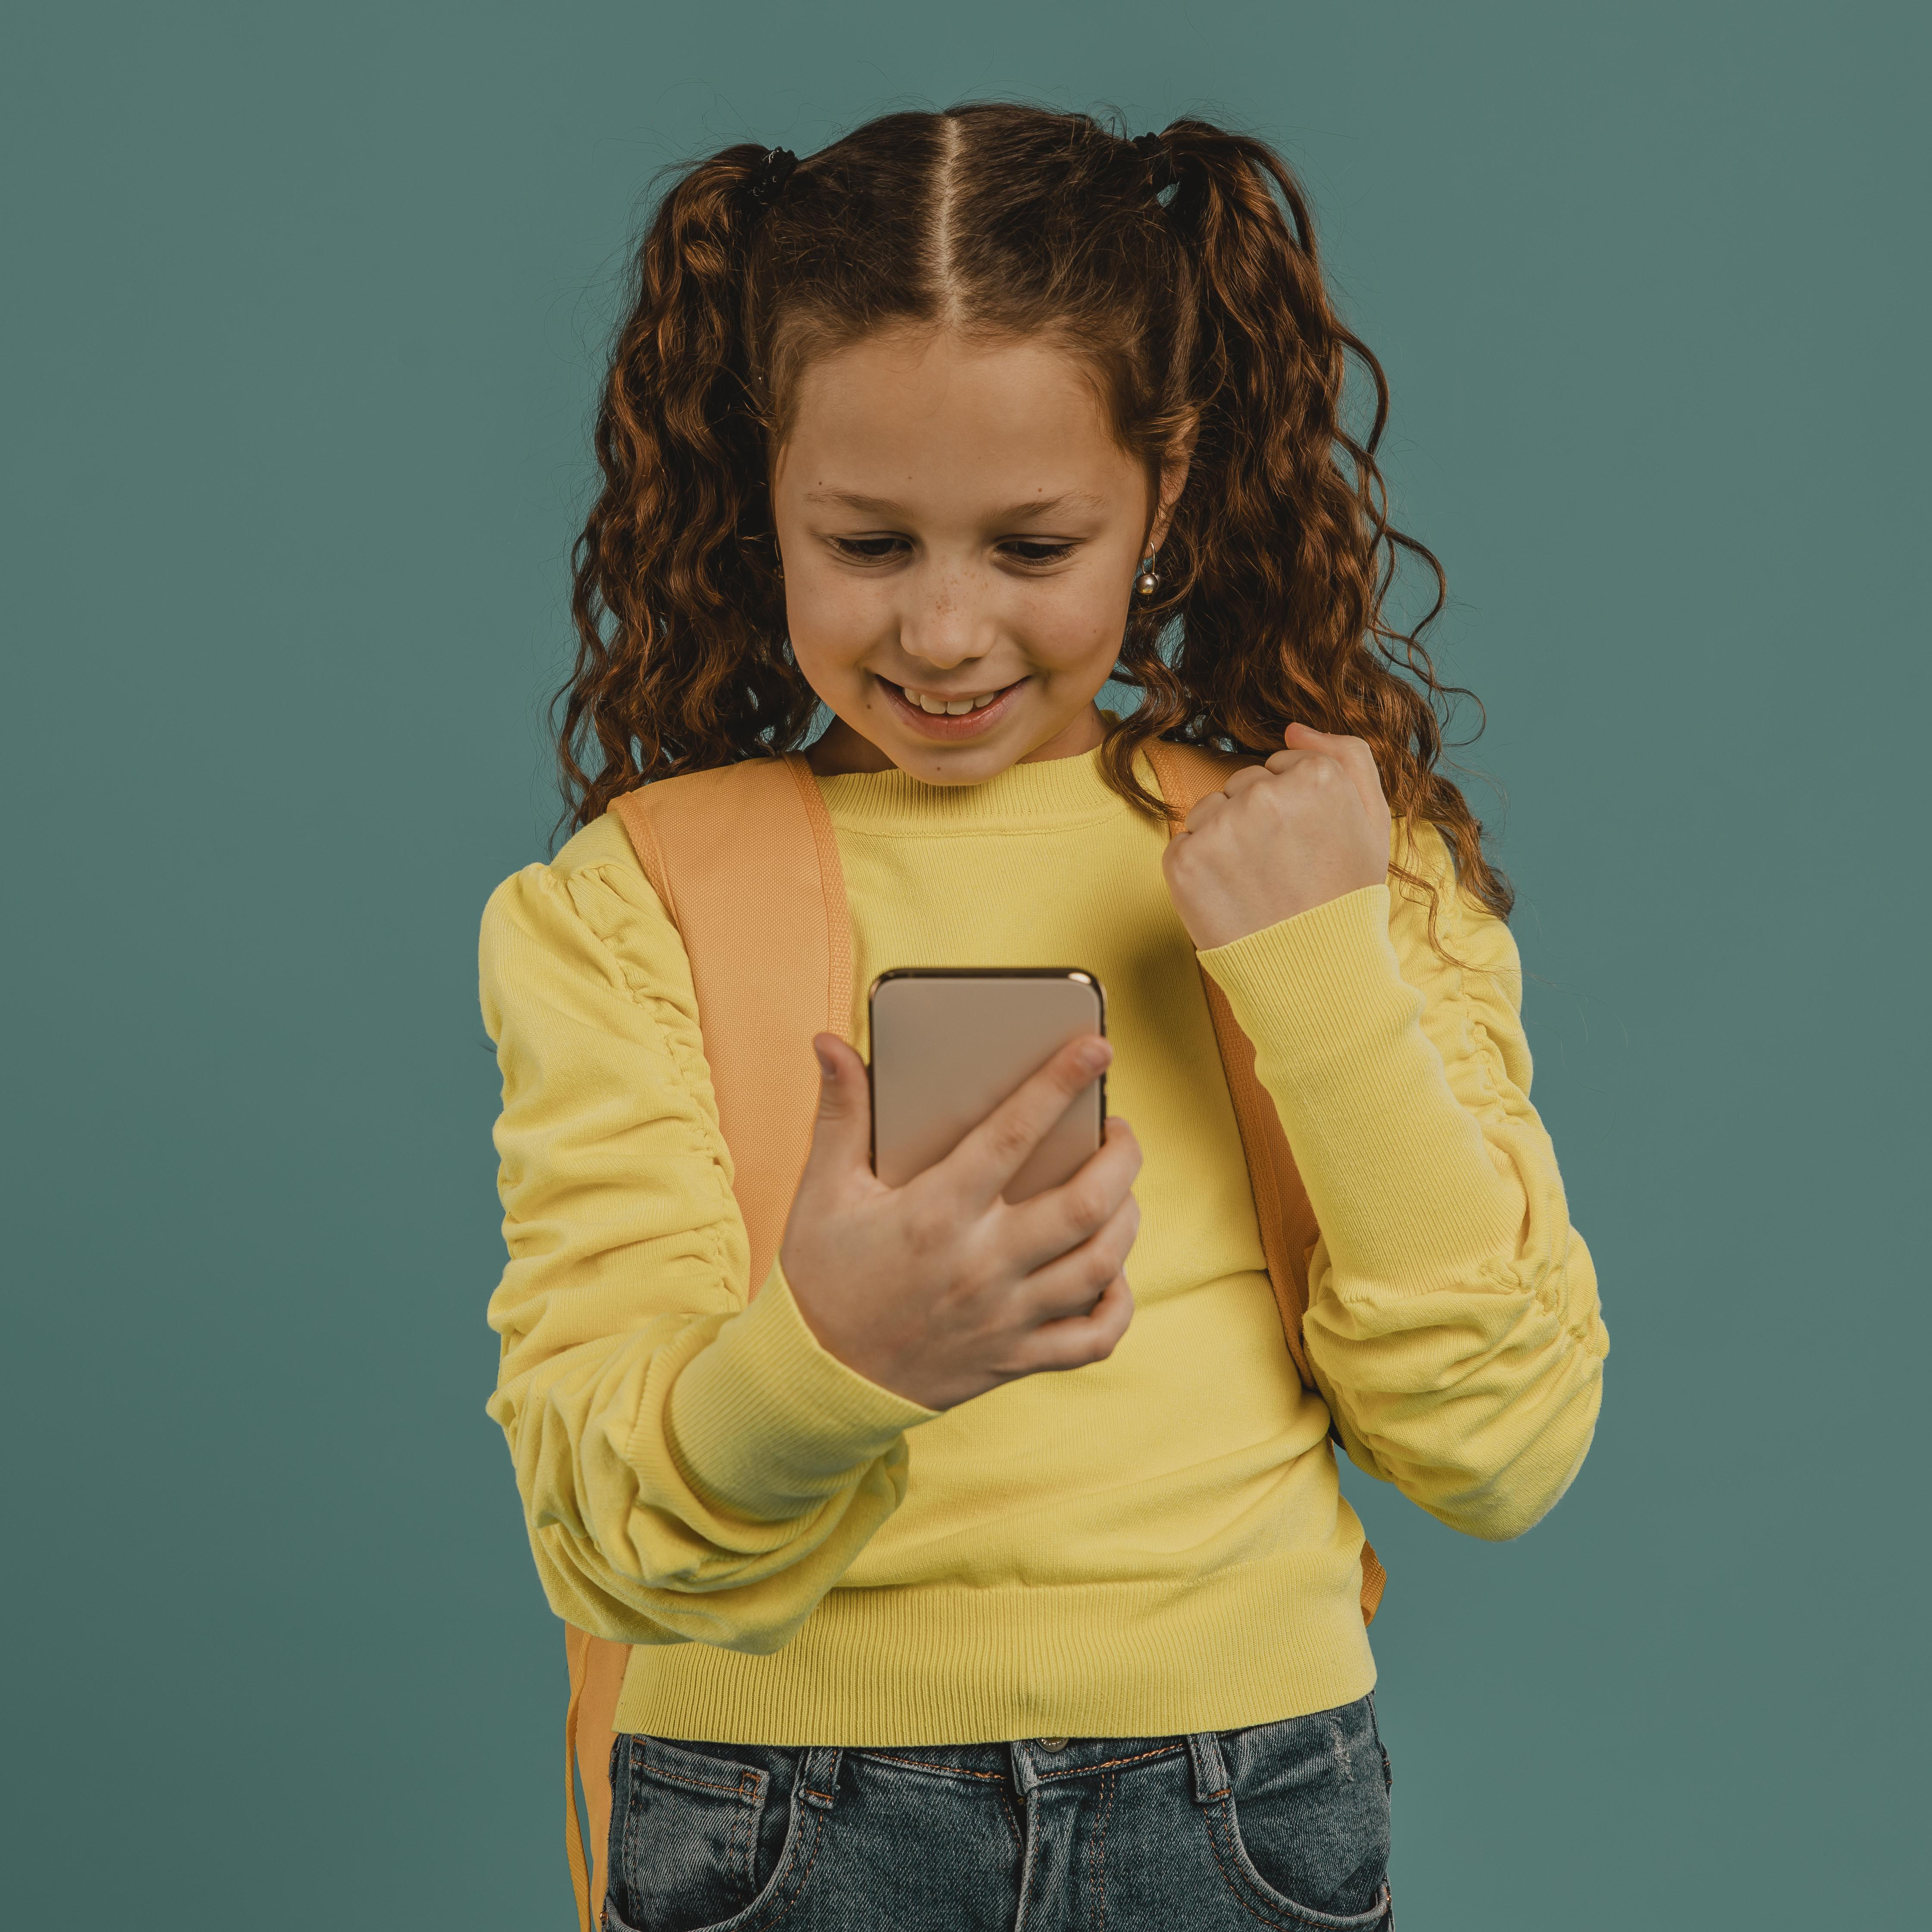
\includegraphics[width=0.9\textwidth]{img3.jpg}} 
            \\[0.3cm]
            \tiny\textcolor{cpsgray}{Fonte: Imagem gerada por IA (Freepik), 2025}
        \end{column}
        
        \begin{column}{0.6\textwidth}
            \justifying
            \textbf{Plataforma de Jogos Educacionais para Crianças com TDAH (2020)}
            \begin{itemize}
                \item Sistema baseado em jogos e quebra-cabeças que estimulam memória, linguagem e pensamento;
                
                \item Software auxiliou positivamente alunos com TDAH com dificuldades em aulas remotas tradicionais;
                
                \item Limitações: alto consumo de memória e versão gratuita com conteúdo limitado/repetitivo;
            \end{itemize}
        \end{column}
    \end{columns}
\end{frame}

% --- Frame estado da arte

\begin{frame}{Estado da arte}
\begin{columns}
        \begin{column}{0.6\textwidth}
            \justifying
            \textbf{App para Pré-Diagnóstico de TEA em crianças (2023)}
            \begin{itemize}
    \item Software analisa dados do Q-CHAT-10 para gerar pré-diagnóstico de TEA;
    
    \item Alta precisão (90,7\%) e sensibilidade (92,6\%) na identificação correta de casos;
    
    \item Comparação feita em grupos que possuem e não possuem TEA;
\end{itemize}
        \end{column}
         \begin{column}{0.35\textwidth}
            \centering
            \fbox{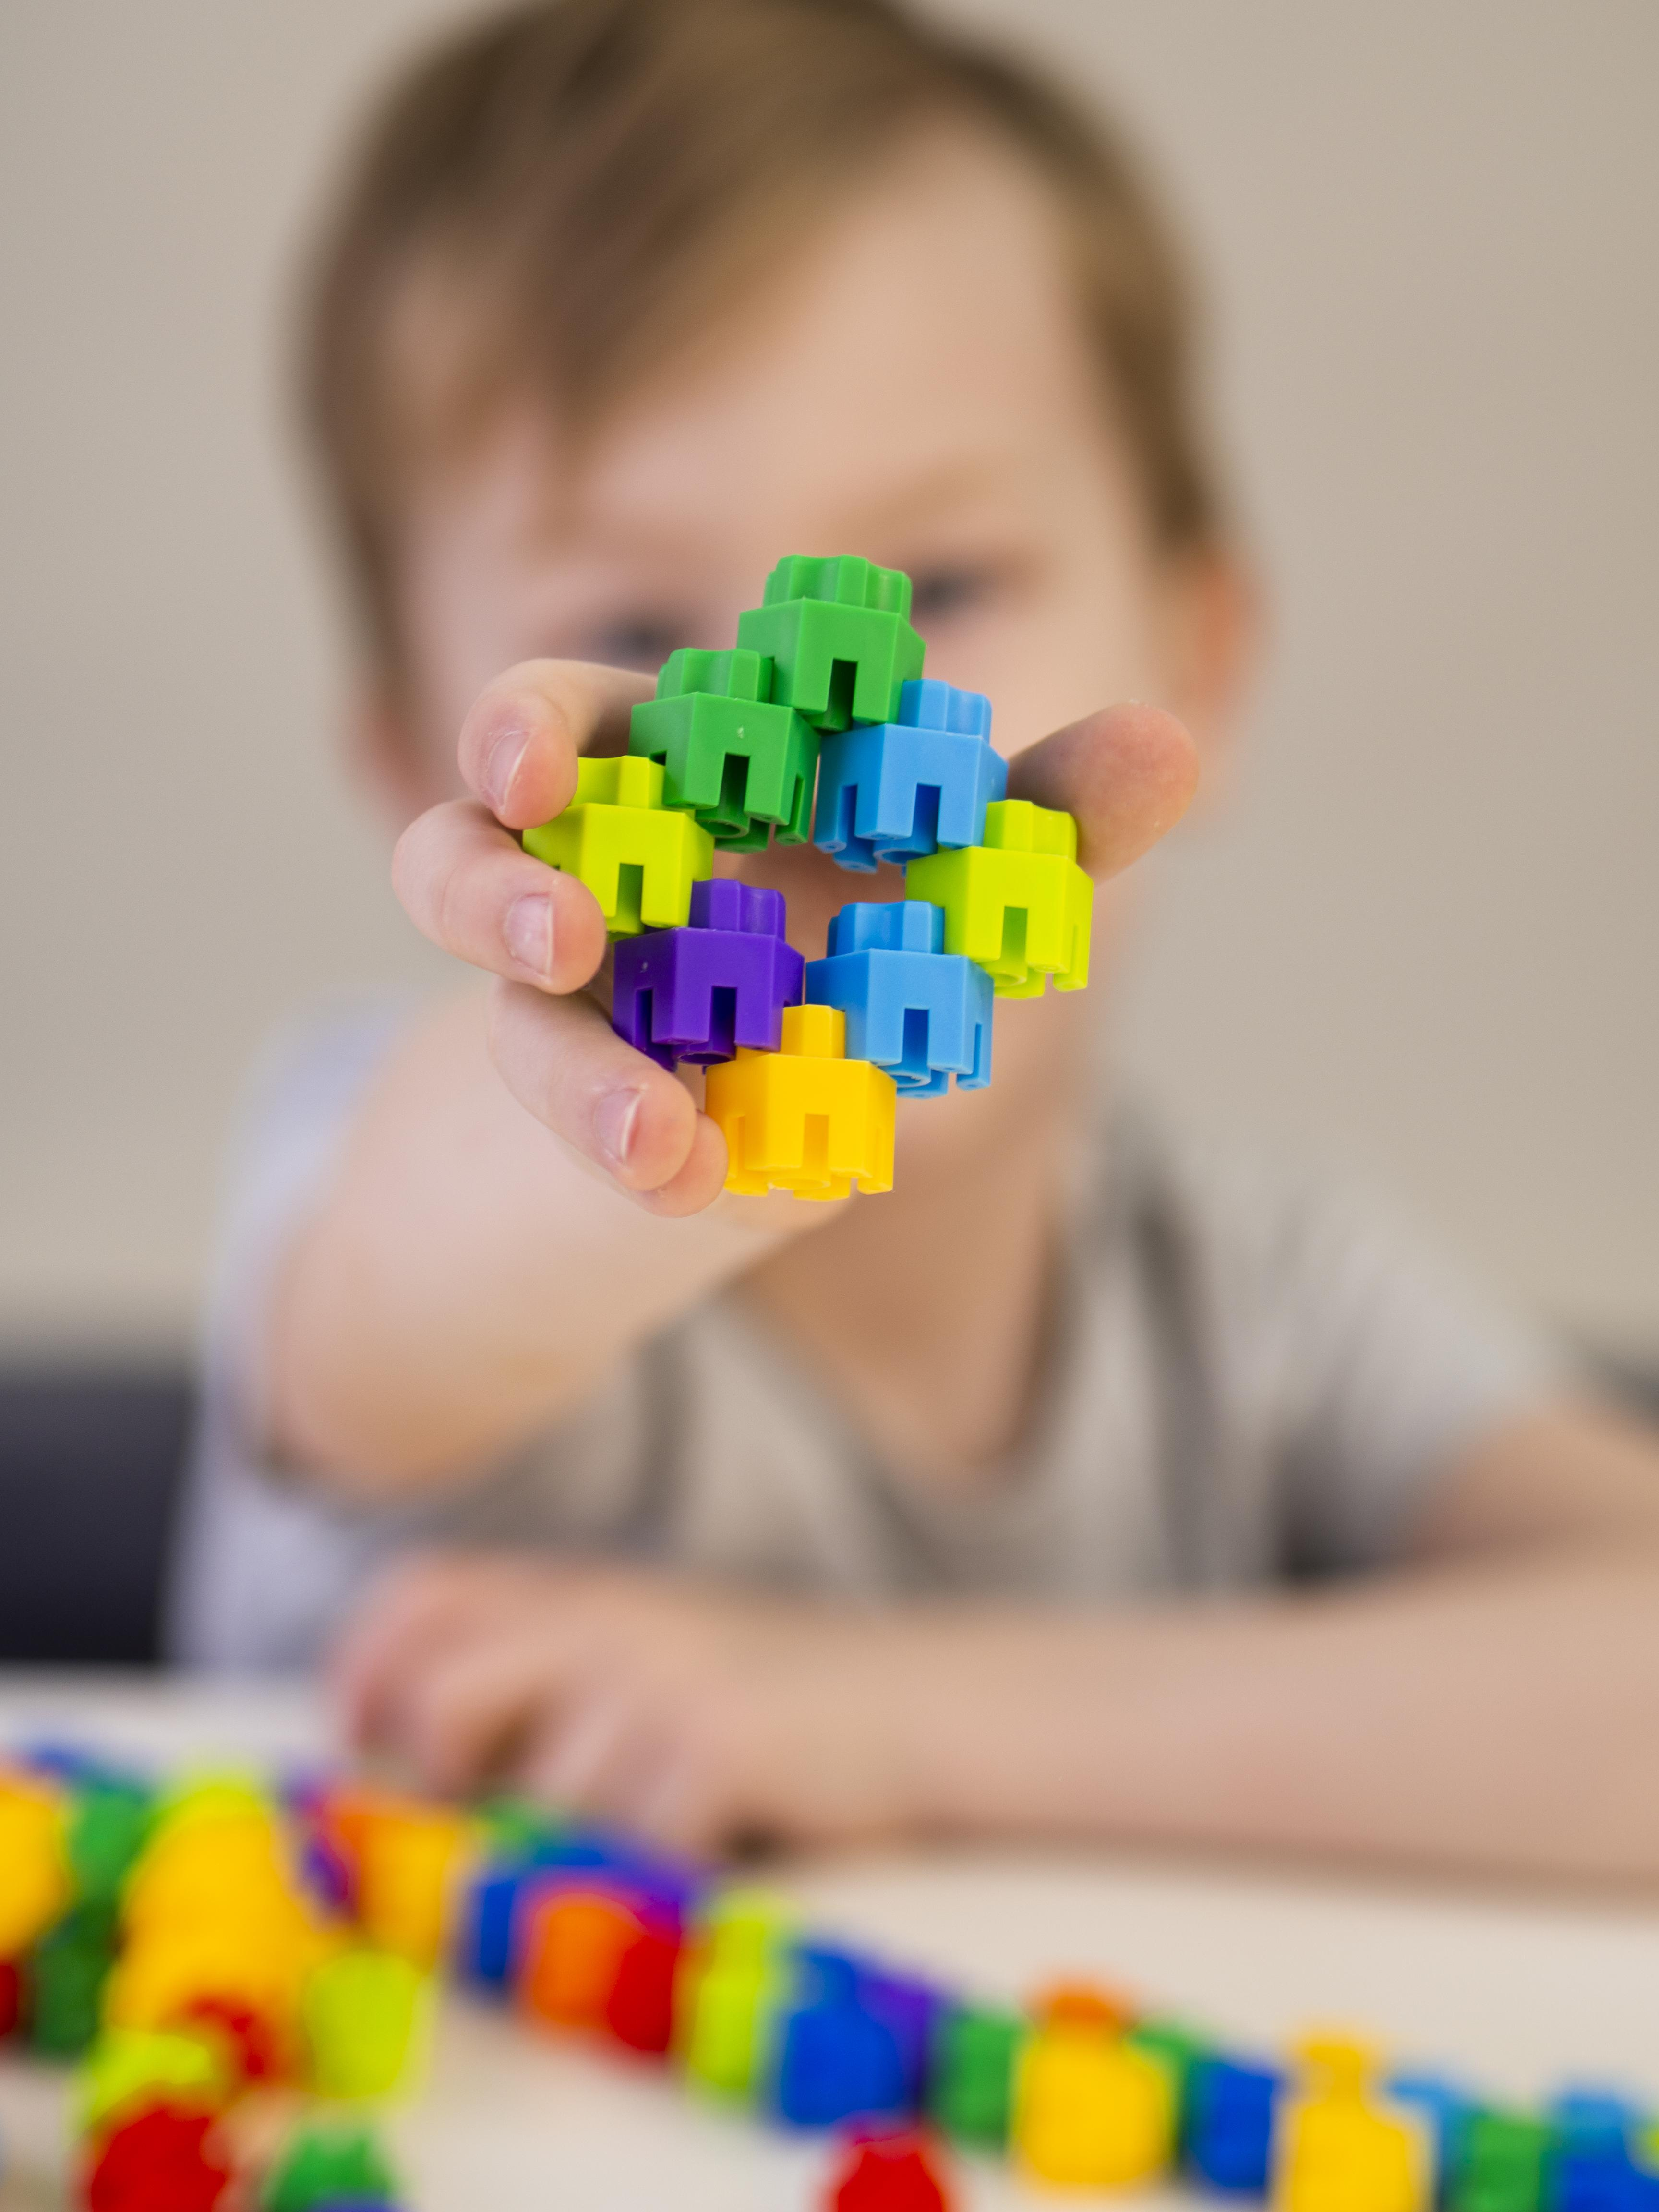
\includegraphics[width=0.9\textwidth]{img4.jpg}} 
            \\[0.3cm]
            \tiny\textcolor{cpsgray}{Fonte: Imagem gerada por IA (Freepik), 2025}Fonte: Imagem gerada por IA (Freepik),
        \end{column}
        
    \end{columns}
\end{frame}

% --- Frame estado da arte

\begin{frame}{Estado da arte}
\begin{columns}
        \begin{column}{0.35\textwidth}
            \centering
            \fbox{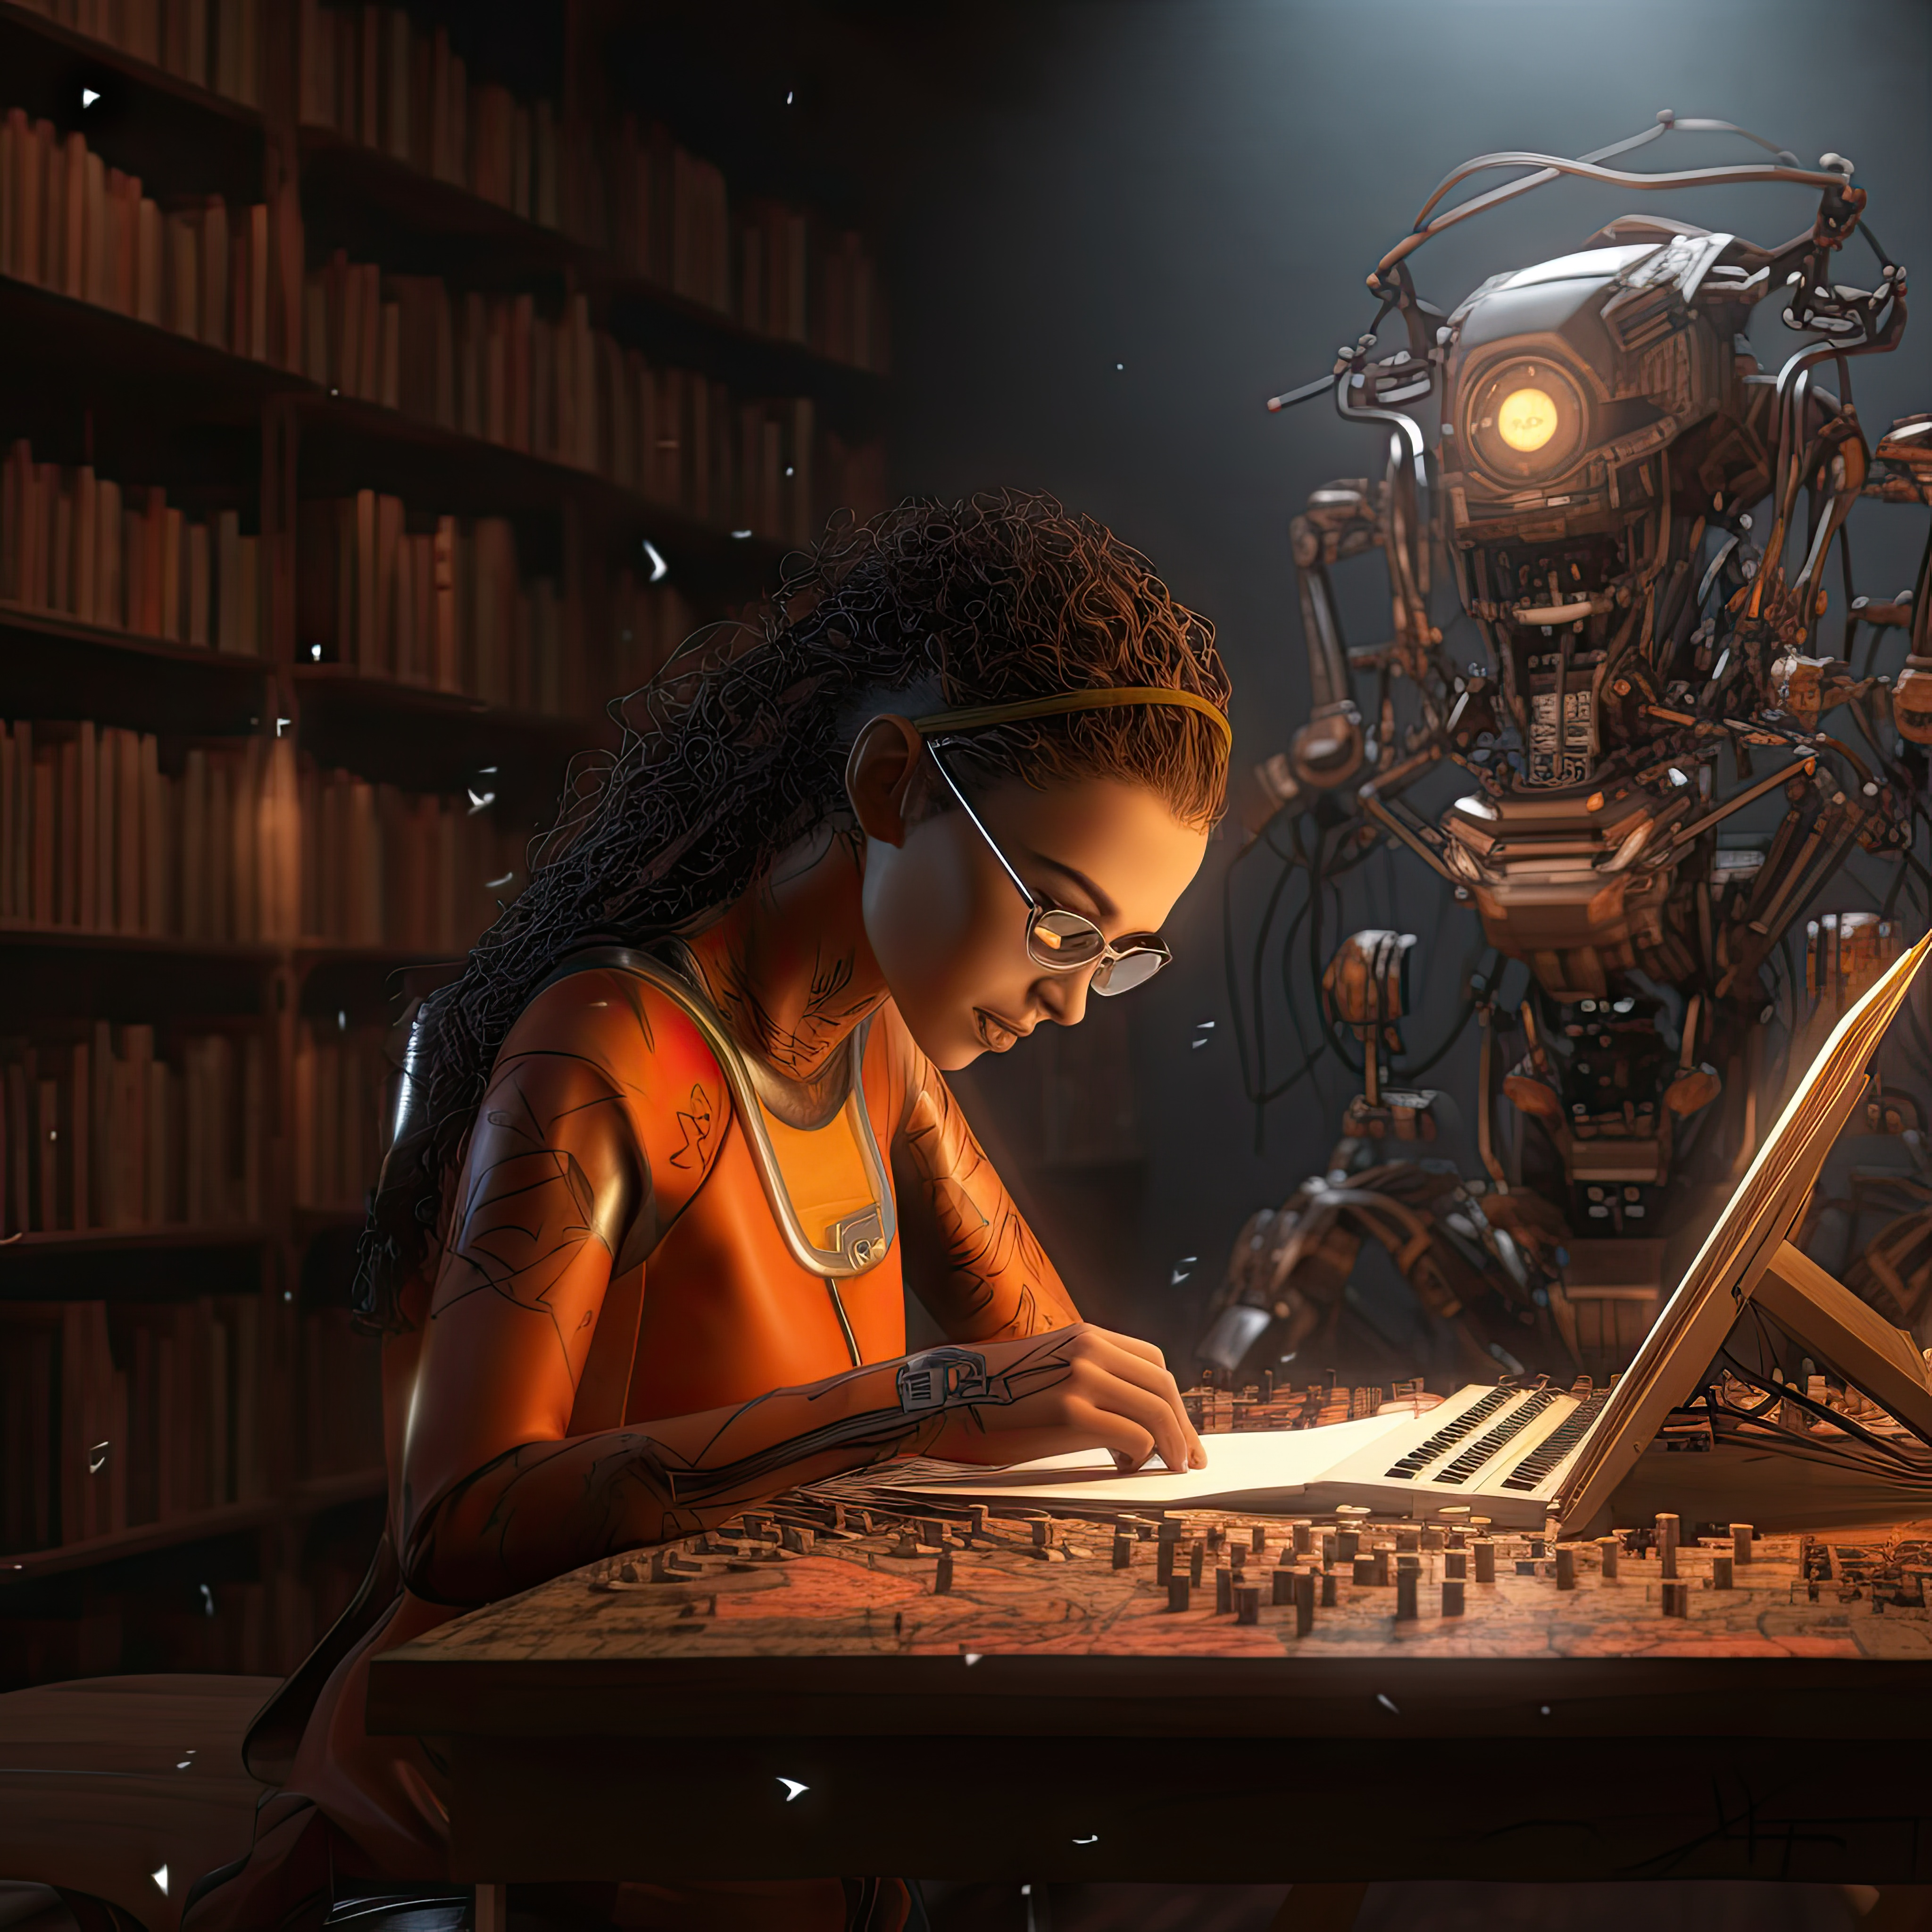
\includegraphics[width=0.9\textwidth]{img5.jpg}} 
            \\[0.3cm]
            \tiny\textcolor{cpsgray}{Fonte: Imagem gerada por IA (Freepik), 2025}
        \end{column}
        
        \begin{column}{0.6\textwidth}
            \justifying
            \textbf{IA Generativa no EAD: Personalização e Aceleração do Aprendizado (2024)}
            \begin{itemize}
    \item Assistente com IA generativa para criação de exercícios e feedback corretivo personalizado;
    
    \item Estudo comparativo mensal: usuários do software x grupo de controle em EAD tradicional;
    
    \item Aumento de (46\%) no progresso, elevando desempenho de (24,1\%) para (69,9\%);
\end{itemize}
        \end{column}
    \end{columns}
\end{frame}

% --- Frame objetivo

\section{Objetivo}
\begin{frame}{Objetivo}
    \begin{columns}[T]
        \begin{column}{0.6\textwidth}
            \begin{tcolorbox}[
                enhanced, colback=white, colframe=cpsred, arc=5mm, boxrule=1.2pt, sharp corners=downhill, width=\linewidth, center, fontupper=\justifying\large, left=10pt, right=10pt, top=10pt, bottom=10pt, shadow={1mm}{-1mm}{0mm}{cpsgray!40},
            ]
                \textbf{\color{cpsred}Objetivo Geral}\par\vspace{0.3cm}
                Adaptar planos de aula do ensino fundamental I de forma lúdica, 
                criando um ambiente visual personalizado através de 
                \textbf{Inteligência Artificial Generativa (IA Generativa)} 
                para crianças de 6 a 10 anos de idade que possuam diagnóstico de TDAH.
            \end{tcolorbox}
        \end{column}
        \begin{column}{0.35\textwidth}
            \centering
            \fbox{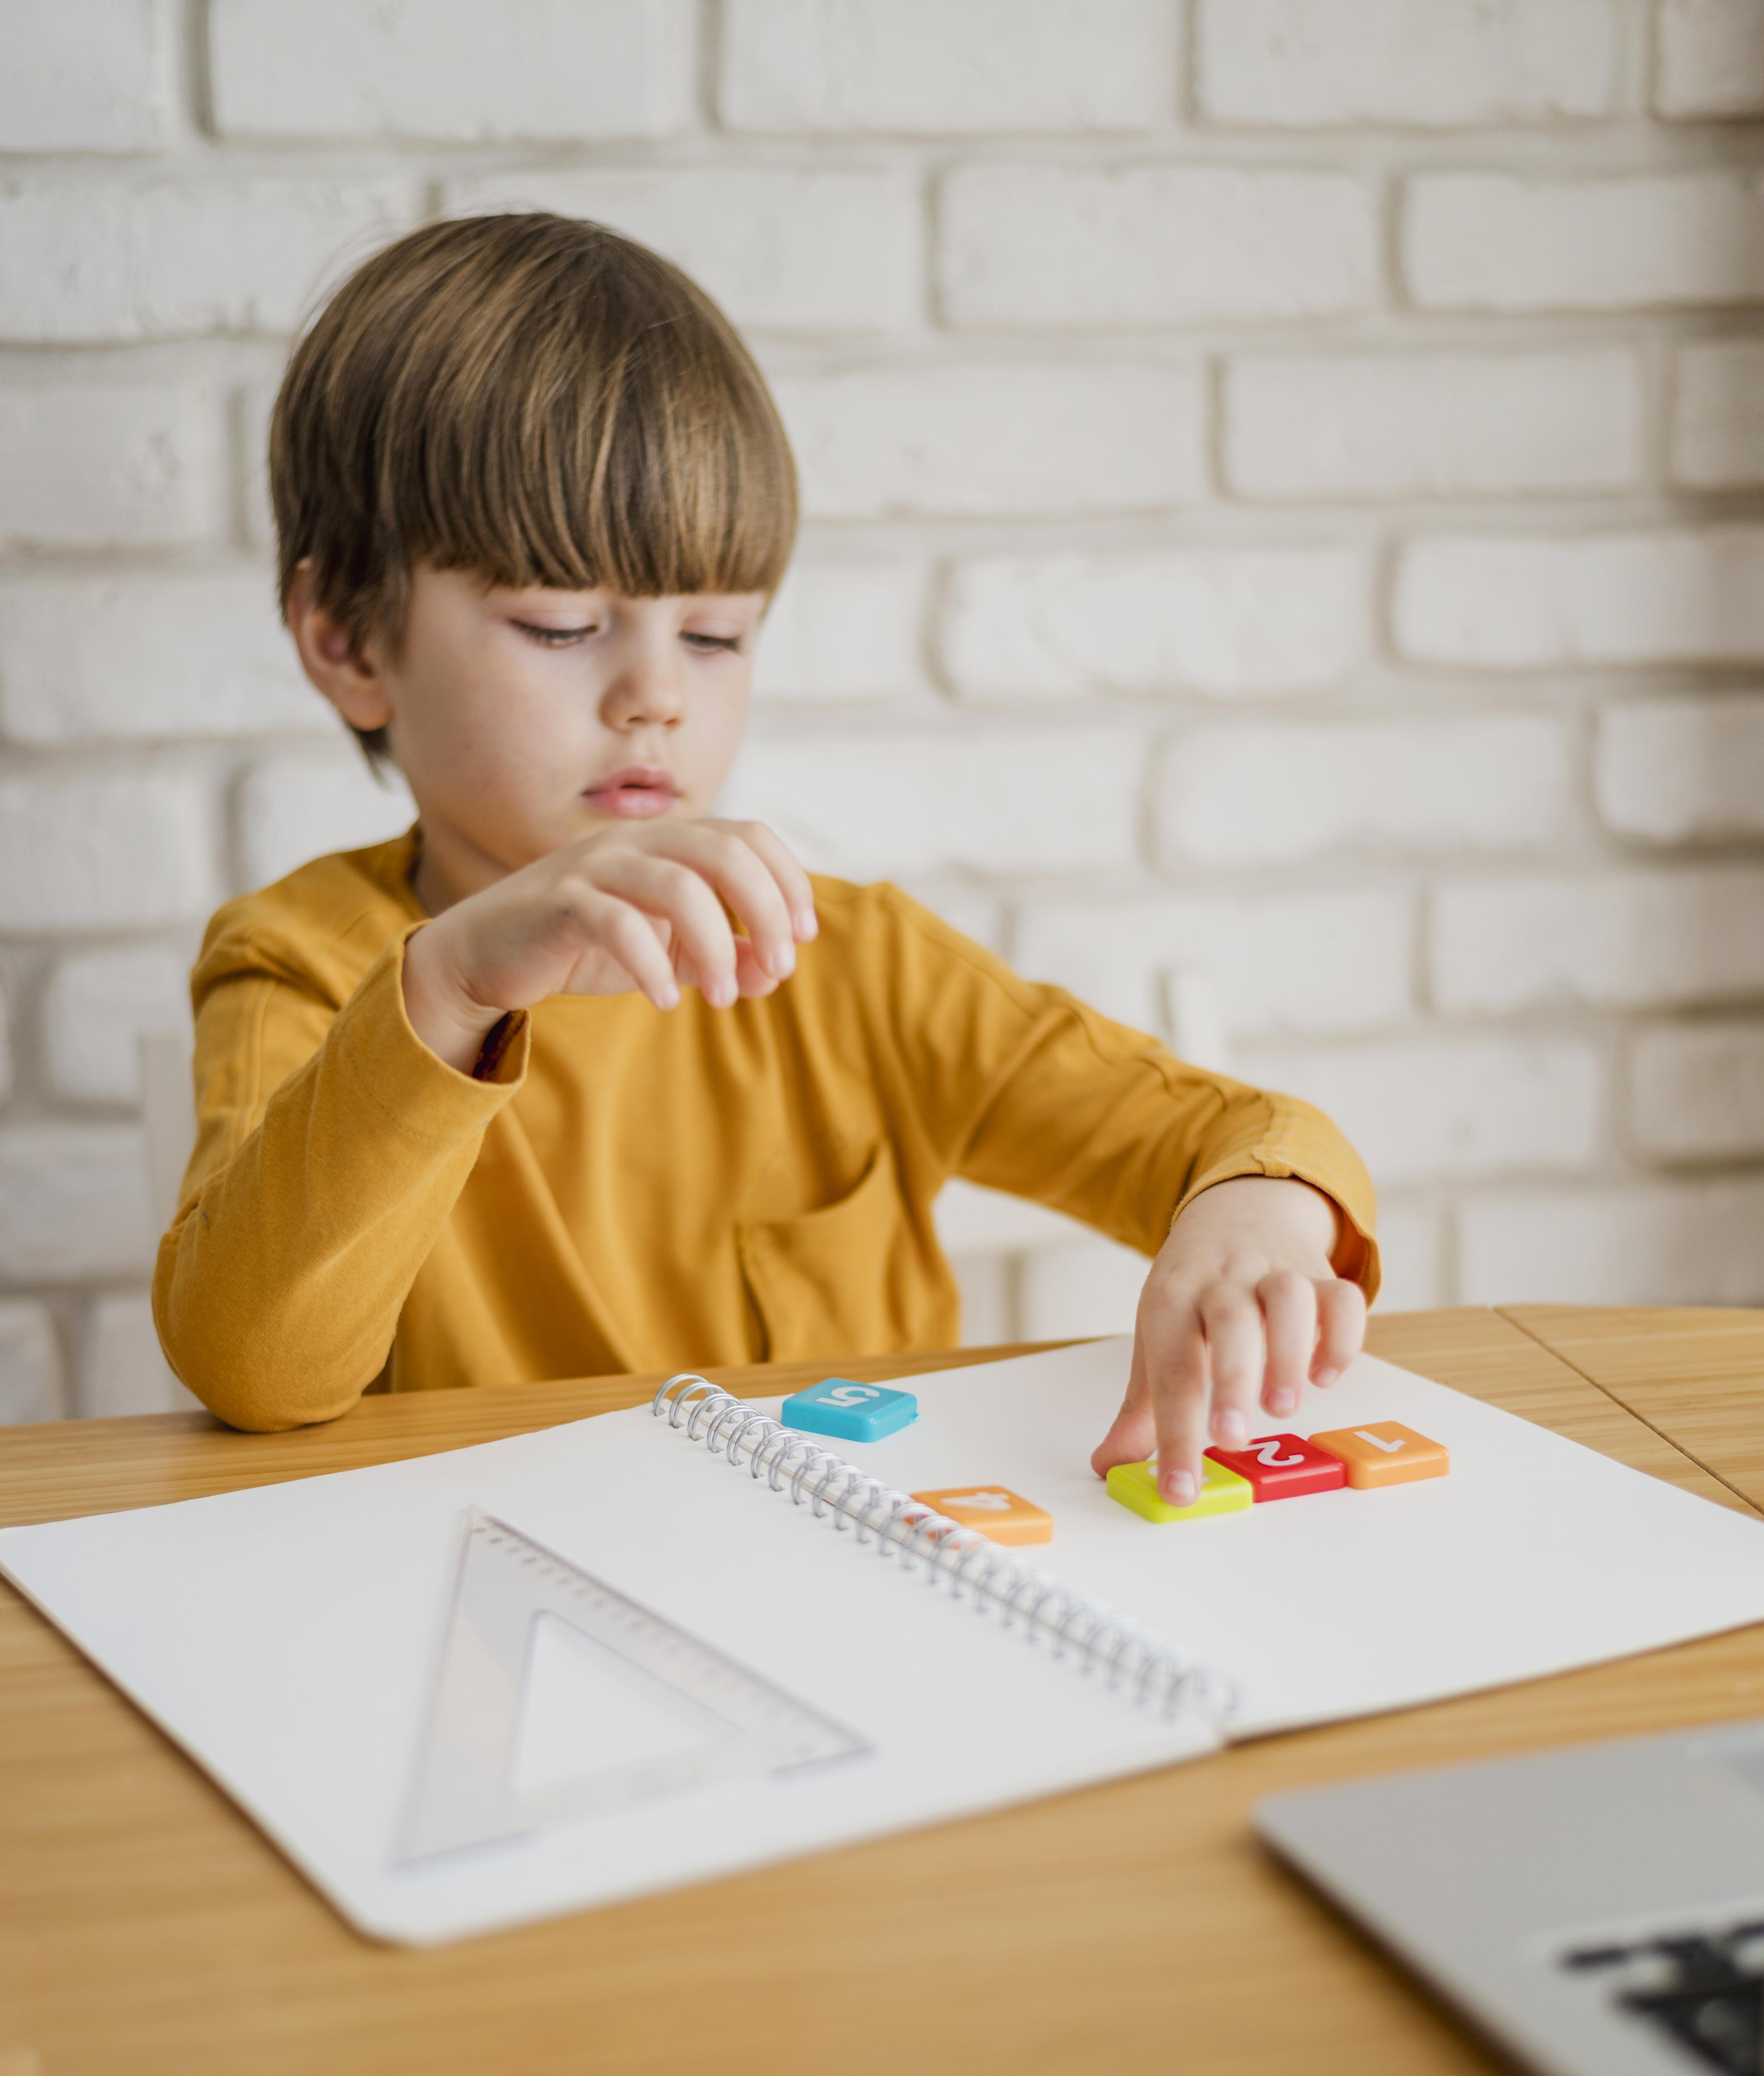
\includegraphics[width=0.9\textwidth]{img2.jpg}} 
            \\[0.3cm]
            \tiny\textcolor{cpsgray}{Fonte: Imagem gerada por IA (Freepik), 2025}
        \end{column}
    \end{columns}
\end{frame}

% --- Frame apresentação prática

\section{Apresentação prática}
\begin{frame}{Apresentação prática}
    \centering
    {\Large\textbf{\textcolor{cpsred}{Demonstração do Projeto Luna}}}\\[0.5cm]
    
   \centering
   {\small  Agora nós iremos mostrar o protótipo da aplicação mobile e o nosso projeto web na prática.}\\[0.5cm]
    
    \vspace{0.2cm}
    
    \begin{center}
        \begin{tcolorbox}[
            enhanced,
            colback=white,
            colframe=cpsred,
            arc=4mm,
            boxrule=1.5pt,
            shadow={2mm}{-1mm}{0mm}{cpsgray!50},
            width=0.8\linewidth,
            center,
            before skip=0.5cm,
            after skip=0.5cm
        ]
        \centering
        \large
        \href{https://www.figma.com/design/HB50qhAAMrpEkTEfcGznwZ/Projeto-Integrador?node-id=18-4&t=4vMySIzPoZhpcH7C-1}{\textbf{UX/UI Mobile}}
        \end{tcolorbox}
        
        \begin{tcolorbox}[
            enhanced,
            colback=white,
            colframe=cpsred,
            arc=4mm,
            boxrule=1.5pt,
            shadow={2mm}{-1mm}{0mm}{cpsgray!50},
            width=0.8\linewidth,
            center,
            before skip=0.5cm,
            after skip=0.5cm
        ]
        \centering
        \large
        \href{http://localhost:8080/}{\textbf{WEB}}
        \end{tcolorbox}
    \end{center}
\end{frame}

% --- Frame agradecimento

\section{Agradecimentos}
\begin{frame}{Agradecimentos}
\centering
    \vspace{1cm}
    
    {\color{cpsred}\Huge\textbf{Obrigado pela atenção!}}\\[1.5cm]
    \textcolor{cpsgray}{\large Centro Paula Souza}\\[0.2cm]
    \textcolor{cpsgray}{\large FATEC Registro}
\end{frame}

\end{document}